\documentclass[11pt,letterpaper]{article}
\usepackage[utf8]{inputenc}
\usepackage[left=1in,right=1in,top=1in,bottom=1in]{geometry}
\usepackage{amsfonts,amsmath,amsthm}
\usepackage{graphicx,float}
% -----------------------------------
\usepackage{hyperref}
\hypersetup{%
  colorlinks=true,
  linkcolor=blue,
  citecolor=blue,
  urlcolor=blue,
  linkbordercolor={0 0 1}
}
% -----------------------------------
\usepackage[style=authoryear,backend=biber]{biblatex}
\addbibresource{citation.bib}
% -----------------------------------
\usepackage{fancyhdr}
\newcommand\course{MATH-UA.0325\\Analysis}
\newcommand\hwnumber{7}                  % <-- homework number
\newcommand\NetIDa{Ryan Sh\`iji\'e D\`u} 
\newcommand\NetIDb{October 24th, 2024}
\pagestyle{fancyplain}
\headheight 35pt
\lhead{\NetIDa\\\NetIDb}
\chead{\textbf{\Large Worksheet \hwnumber}}
\rhead{\course}
\lfoot{}
\cfoot{}
\rfoot{\small\thepage}
\headsep 1.5em
% -----------------------------------
\usepackage{titlesec}
\renewcommand\thesubsection{(\arabic{section}.\alph{subsection})}
\titleformat{\subsection}[runin]
        {\normalfont\bfseries}
        {\thesubsection}% the label and number
        {0.5em}% space between label/number and subsection title
        {}% formatting commands applied just to subsection title
        []% punctuation or other commands following subsection title
% -----------------------------------
\setlength{\parindent}{0.0in}
\setlength{\parskip}{0.1in}
% -----------------------------------
\newcommand{\de}{\mathrm{d}}
\newcommand{\DD}{\mathrm{D}}
\newcommand{\pe}{\partial}
\newcommand{\mcal}{\mathcal}
%\newcommand{\pdx}{\left|\frac{\partial}{\partial_x}\right|}

\newcommand{\dsp}{\displaystyle}

\newcommand{\norm}[1]{\left\Vert #1 \right\Vert}
%\newcommand{\mean}[1]{\left\langle #1 \right\rangle}
\newcommand{\mean}[1]{\overline{#1}}
\newcommand{\inner}[2]{\left\langle #1,#2\right\rangle}

\newcommand{\ve}[1]{\boldsymbol{#1}}

\newcommand{\thus}{\Rightarrow \quad }
\newcommand{\fff}{\iff\quad}
\newcommand{\qdt}[1]{\quad \mbox{#1} \quad}

\renewcommand{\Re}{\mathrm{Re}}
\renewcommand{\Im}{\mathrm{Im}}
\newcommand{\E}{\mathbb{E}}
\newcommand{\lap} {\nabla^2}
\renewcommand{\div}{\nabla\cdot}

\newcommand{\csch}{\text{csch}}
\newcommand{\sech}{\text{sech}}


\newcommand{\hot}{\text{h.o.t.}}

\newcommand{\ssp}{\left.\qquad\right.}

\newcommand{\var}{\text{var}}
\newcommand{\cov}{\text{cov}}

%%%%%%%%%%%%%%%%%%%%%%%%%%%%%%%%%%%%%%%%%%%%%%%%%%
\makeatletter
\newcommand*{\mint}[1]{%
  % #1: overlay symbol
  \mint@l{#1}{}%
}
\newcommand*{\mint@l}[2]{%
  % #1: overlay symbol
  % #2: limits
  \@ifnextchar\limits{%
    \mint@l{#1}%
  }{%
    \@ifnextchar\nolimits{%
      \mint@l{#1}%
    }{%
      \@ifnextchar\displaylimits{%
        \mint@l{#1}%
      }{%
        \mint@s{#2}{#1}%
      }%
    }%
  }%
}
\newcommand*{\mint@s}[2]{%
  % #1: limits
  % #2: overlay symbol
  \@ifnextchar_{%
    \mint@sub{#1}{#2}%
  }{%
    \@ifnextchar^{%
      \mint@sup{#1}{#2}%
    }{%
      \mint@{#1}{#2}{}{}%
    }%
  }%
}
\def\mint@sub#1#2_#3{%
  \@ifnextchar^{%
    \mint@sub@sup{#1}{#2}{#3}%
  }{%
    \mint@{#1}{#2}{#3}{}%
  }%
}
\def\mint@sup#1#2^#3{%
  \@ifnextchar_{%
    \mint@sup@sub{#1}{#2}{#3}%
  }{%
    \mint@{#1}{#2}{}{#3}%
  }%
}
\def\mint@sub@sup#1#2#3^#4{%
  \mint@{#1}{#2}{#3}{#4}%
}
\def\mint@sup@sub#1#2#3_#4{%
  \mint@{#1}{#2}{#4}{#3}%
}
\newcommand*{\mint@}[4]{%
  % #1: \limits, \nolimits, \displaylimits
  % #2: overlay symbol: -, =, ...
  % #3: subscript
  % #4: superscript
  \mathop{}%
  \mkern-\thinmuskip
  \mathchoice{%
    \mint@@{#1}{#2}{#3}{#4}%
        \displaystyle\textstyle\scriptstyle
  }{%
    \mint@@{#1}{#2}{#3}{#4}%
        \textstyle\scriptstyle\scriptstyle
  }{%
    \mint@@{#1}{#2}{#3}{#4}%
        \scriptstyle\scriptscriptstyle\scriptscriptstyle
  }{%
    \mint@@{#1}{#2}{#3}{#4}%
        \scriptscriptstyle\scriptscriptstyle\scriptscriptstyle
  }%
  \mkern-\thinmuskip
  \int#1%
  \ifx\\#3\\\else_{#3}\fi
  \ifx\\#4\\\else^{#4}\fi  
}
\newcommand*{\mint@@}[7]{%
  % #1: limits
  % #2: overlay symbol
  % #3: subscript
  % #4: superscript
  % #5: math style
  % #6: math style for overlay symbol
  % #7: math style for subscript/superscript
  \begingroup
    \sbox0{$#5\int\m@th$}%
    \sbox2{$#5\int_{}\m@th$}%
    \dimen2=\wd0 %
    % => \dimen2 = width of \int
    \let\mint@limits=#1\relax
    \ifx\mint@limits\relax
      \sbox4{$#5\int_{\kern1sp}^{\kern1sp}\m@th$}%
      \ifdim\wd4>\wd2 %
        \let\mint@limits=\nolimits
      \else
        \let\mint@limits=\limits
      \fi
    \fi
    \ifx\mint@limits\displaylimits
      \ifx#5\displaystyle
        \let\mint@limits=\limits
      \fi
    \fi
    \ifx\mint@limits\limits
      \sbox0{$#7#3\m@th$}%
      \sbox2{$#7#4\m@th$}%
      \ifdim\wd0>\dimen2 %
        \dimen2=\wd0 %
      \fi
      \ifdim\wd2>\dimen2 %
        \dimen2=\wd2 %
      \fi
    \fi
    \rlap{%
      $#5%
        \vcenter{%
          \hbox to\dimen2{%
            \hss
            $#6{#2}\m@th$%
            \hss
          }%
        }%
      $%
    }%
  \endgroup
}

\begin{document}

\section{} 
\subsection{}[Exercise 3.1.9 of \cite{Lebl_23}] 
Let $c_1$ be a cluster point of $A\subset\mathbb{R}$ and $c_2$ be a cluster point of $B\subset\mathbb{R}$. Suppose $f:A\to B$
and $g:B\to \mathbb{R}$ are functions such that $f(x)\to c_2$ as $x\to c_1$ and $g(y)\to L$ as $y\to c_2$. 

Let $h(x):= g(f(x))$, we have ``chain rule'' for limits: $h(x)\to L$ as $x\to c_1$, if we also suppose that $g(c_2)=L$ (that is, $g(x)$ is continuous at $c_2$).

\subsection{}[Exercise 3.1.14 of \cite{Lebl_23}] 
Show via a counterexample that the assumption of $g(c_2)=L$ is necessary.

\section{} [Exercise 3.2.1 of \cite{Lebl_23}] 
Using the definition of continuity directly prove that $f: \mathbb{R}\to \mathbb{R}$ defined by $f(x) := x^2$ is continuous.

\section{} [Example 3.2.6 of \cite{Lebl_23}] 
Show that the functions $\sin(x)$ and $\cos(x)$ are continuous. \\
Hint: use the sum-to-product trigonometric identities.

\section{} [Example 3.2.12 of \cite{Lebl_23}] 
Show that the popcorn function (or the Thomae function) is continuous. The popcorn function is defined as $f:(0,1)\to \mathbb{R}$
\begin{align}
    f(x) := \begin{cases}
        1/k & \text{if } x=m/k, \text{ where }m,k\in\mathbb{N}\text{ and have no common divisors,}\\
        0 & \text{if }x\text{ is irrational.}
    \end{cases}
\end{align}

\begin{figure}[H]
    \centering
    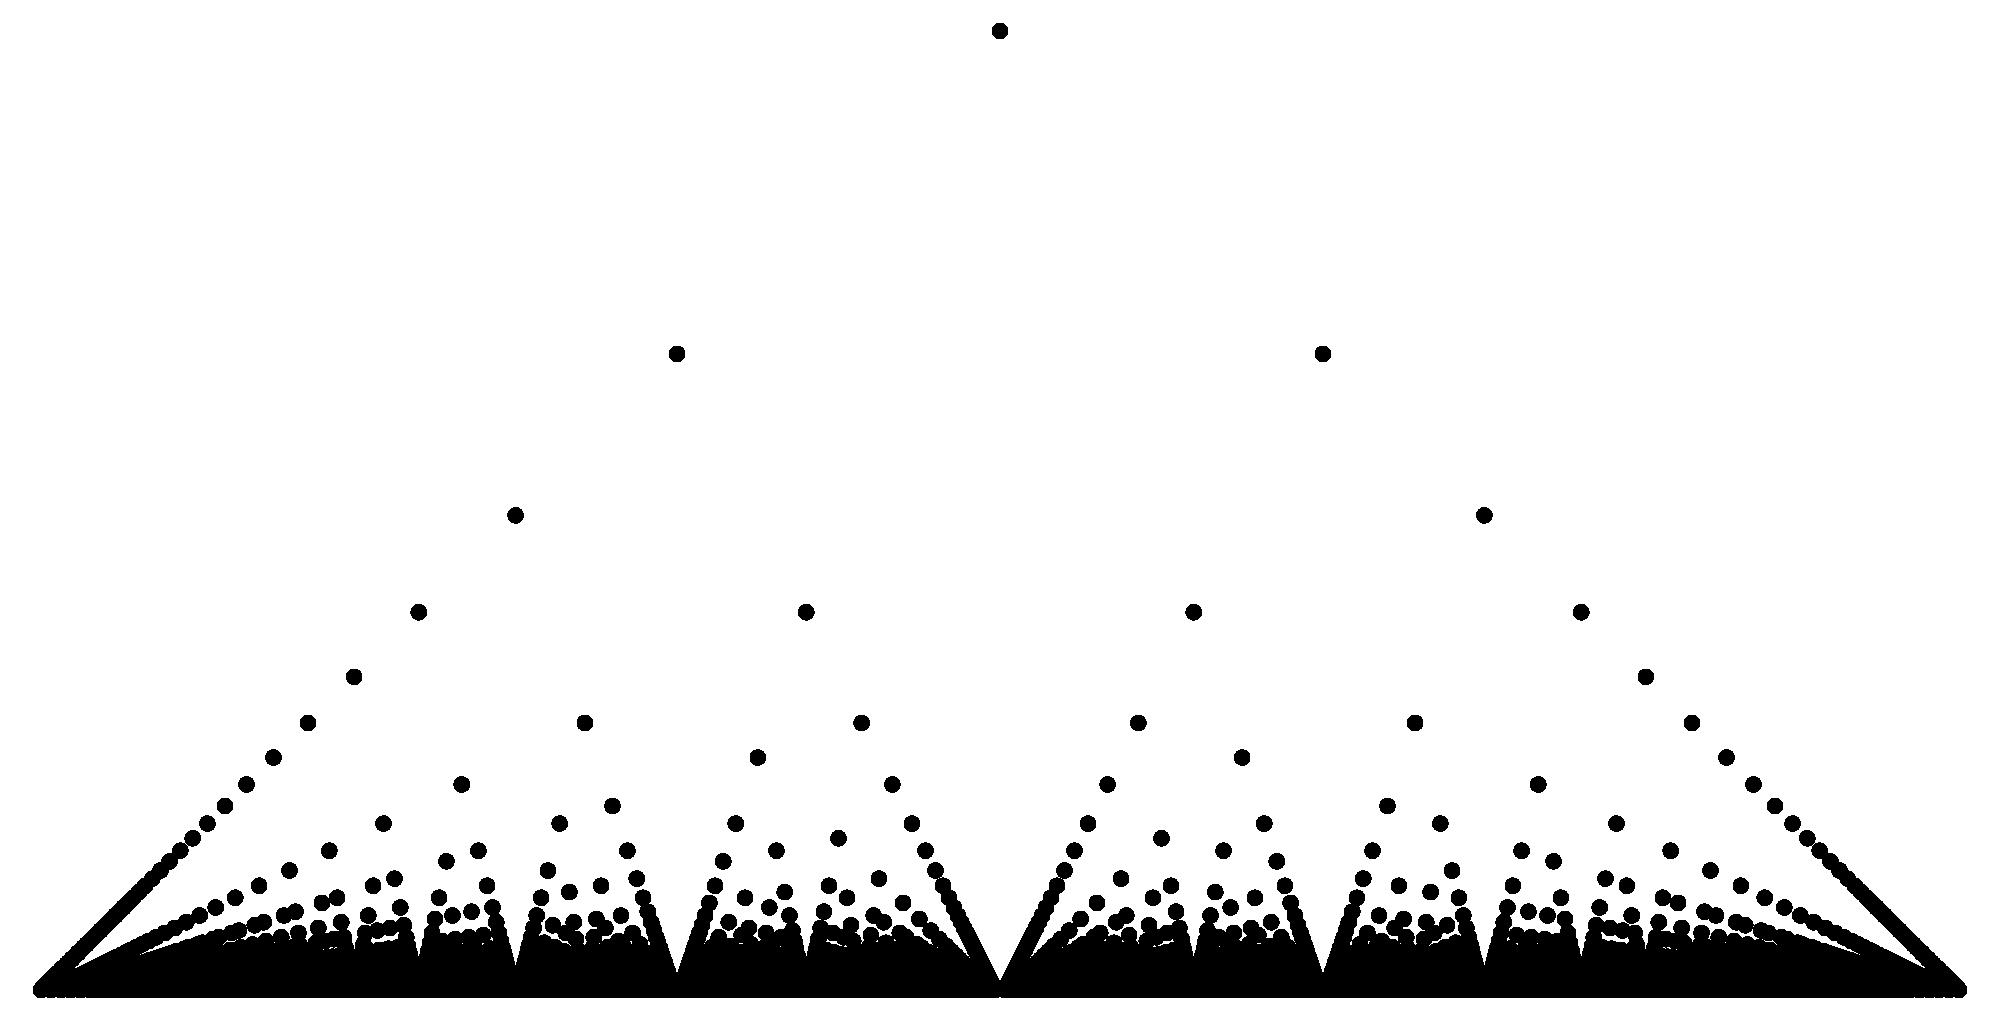
\includegraphics[width=0.5\linewidth]{Thomae_function}
    \caption{Graph of the popcorn function. }
\end{figure}

\section{} [Exercise 3.2.4 and 3.2.4 of \cite{Lebl_23}] 
Is $f: \mathbb{R}\to \mathbb{R}$ continuous? Prove your assertion.

\subsection{}
\begin{align}
    f(x) := \begin{cases}
        \sin(1/x) &\text{if } x\neq 0,\\
        0  &\text{if } x= 0.
    \end{cases}
\end{align}

\subsection{}
\begin{align}
    f(x) := \begin{cases}
        x\sin(1/x) &\text{if } x\neq 0,\\
        0  &\text{if } x= 0.
    \end{cases}
\end{align}

\section{} [Exercise 3.2.10 of \cite{Lebl_23}] 
Let $f:\mathbb{R}\to \mathbb{R}$ and $g:\mathbb{R}\to \mathbb{R}$ be continuous functions. Suppose that $f(r)=g(r)$ for all $r\in\mathbb{Q}$. Show that $f(x)=g(x)$ for all $x\in\mathbb{R}$. 


\vfill
\printbibliography


\end{document}